\documentclass[en]{university}

\faculty{Department of Computer Engineering}
\course{Artificial Intelligence}
\subject{Mini Project 4 Theory Questions}
\professor{Dr. Rohban}
\student{Parsa Mohammadian}

\begin{document}

\setupdocument

\section{}

\subsection{}

\includepdfall{assets/1a.pdf}

\subsection{}

We can use introduced features as nodes of the decision tree, and values (black and white) as the edges of the decision tree. But 
this structure is extremely over fitted to the data. We can traverse resulting tree to classify the input image $X$ but it is not 
accurate.

\section{}



\section{}

Since perceptron is a linear classifier, we can introduce an neural network consisting of multiple layer of perceptrons for the given shape. 
First we find the weights and biases of the first layer of perceptrons as shown in figure \ref{fig:w}. Each $w_i, b_i$ is weight and bias 
of the $P_i$ perceptron in the first layer.

\begin{figure}[!htbp]
\centering
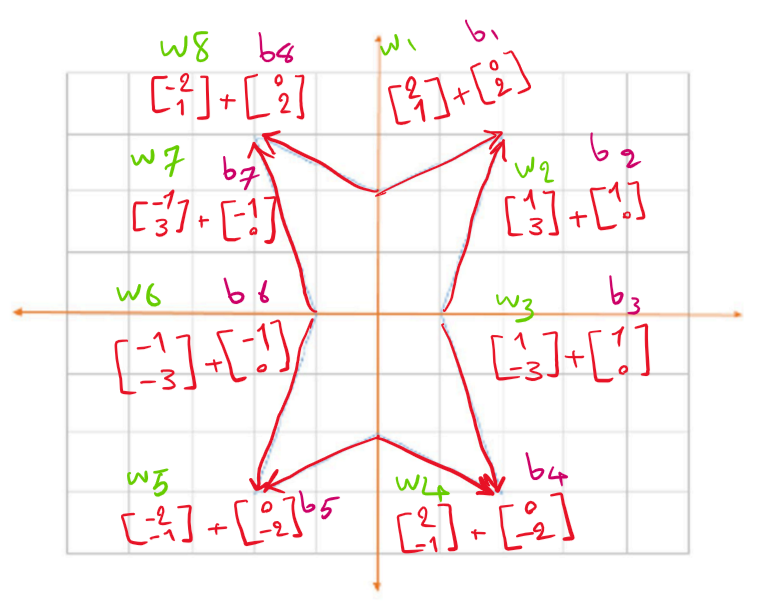
\includegraphics[width=1\textwidth]{assets/3w.png}
\caption{Weights and biases of the first layer of perceptrons}
\label{fig:w}
\end{figure}

with the first layer, our classification become linear, so we use a single perceptron in the second layer. The whole neural network 
is shown in figure \ref{fig:n}.

\begin{figure}
\centering
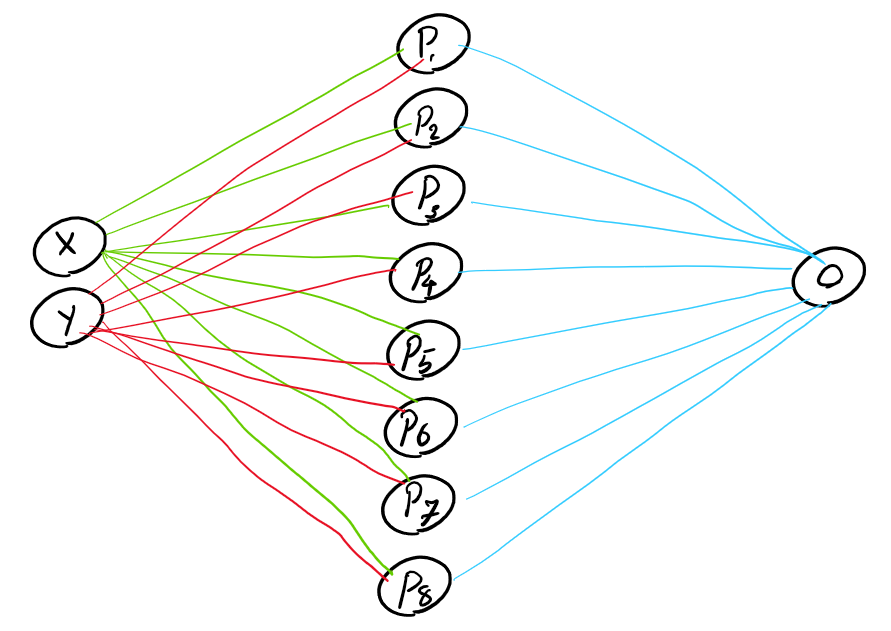
\includegraphics[width=1\textwidth]{assets/3n.png}
\caption{Neural network}
\label{fig:n}
\end{figure}

\end{document}